 \chapter{Analytic approximations and calculations}
\section{Rate equations for leptogenesis}
Now in order to qualitatively describe leptogenesis one has to consider rate equations for the lepton number and B-L number densities. In a static universe without lepton number violating processes the rate equation would trivialy be
\begin{equation}
	\frac{d}{dt}n=0
	\label{eq:rate_static_nointeraction}
\end{equation}
If one now condsiders a universere expandig with the rate H the rate equation above changes to.
\begin{equation}
\left(\frac{d}{dt}+3H\right)n=0
\label{eq:rate_expanding_nointeraction}
\end{equation}
Finally including lepton number violating processes the rate equation one obtains for the neutrino number density is
\begin{equation}
\left(\frac{d}{dt}+3H\right)n_N=-\Gamma_N\left(n_N-n_N^{eq}\right)+\Gamma_{N,B-L}n_{B-L}
\label{eq:L_rate_expanding_interaction}
\end{equation}
Applying this reasoning to the B-L number density yields
\begin{equation}
\left(\frac{d}{dt}+3H\right)n_{B_L}=\Gamma_{B-L,N}\left(n_N-n_N^{eq}\right)+\Gamma_{B-L}n_{B-L}
\label{eq:B-L_rate_expanding_interaction}
\end{equation}
The coefficient $\Gamma_N$ denotes how fast the neutrino density equalizes with its equilibrium density, while $\Gamma_{B-L}$ describes the washout of a net B-L number. $\Gamma_{B-L,N}$ describes how the B-L asymmetry is affected by the deviation of the neutrino density from its equilibrium value and together with $\Gamma_{N,B-L}$ these two coefficients characterize CP violating processes \cite[p. 4]{Bodeker:2013qaa}. Since both these coefficients describe CP violating processes they must depend on the CP violating parameter $\epsilon$ introduced in the section before and it was also seen there that this parameter is small vor heavy neutrino decays and therefore the second term in equation can be neglegted. \newline
The goal now is to determine these coefficients at least at leading order and the first one will be $\Gamma_N$. To get this coefficient one has to integrate equation \ref{eq:L_rate_expanding_interaction} over phase space, resulting in
\begin{equation}
	\left(\frac{\partial}{\partial t}-Hp\frac{\partial}{\partial p}\right)f_N=\Gamma_N\left(e^{E_N/T}-f_N\right)
	\label{eq:boltzmann}
\end{equation}
The whole calculation on how performing the phase space integral can be found in appendix \ref{ap:phase_space}. \newline
One might now notice that equation \ref{eq:boltzmann} differs from equation 4 in \cite{Bodeker:2013qaa} by a factor of $\frac{M_N}{E_N}$, that origins in a different normaliziation of the phase space. However, since we operate in a non-relativistic regime E\textsubscript{N} $\approx$ M\textsubscript{N} and therefore this factor is $\sim$ 1 and negligible. Using this argumentation one can also see that $\Gamma_N=\Gamma_0$ with $\Gamma_0$ the total decay rate of the heavy neutrinos, wich is governed by the Yukawa interaction term \ref{eq:Yukterm}. It has to be mentioined that for the equilibrium distribution the Boltzmann statistic with neglegted chemical potential was used since the energy of a neutrino E\textsubscript{N} $\approx$ M\textsubscript{N} $\gg$ T during the phase where the decay happen outside equilibrium and therefore quantum mechanical effects play an insignificant role and can be neglected. Going back to the decay rate, that can be calculated as done in appendix \ref{ap:tree_level_decay}, one gets
\begin{equation}
\Gamma_N=\Gamma_0=\frac{|h_{11}|^2M_N}{8\pi}
\label{eq:Gamma_N}
\end{equation}
Since the coefficient $\Gamma_{B-L}$ refers to the washout of the B-L asymmetry it arises from the inverse decay l$\phi\rightarrow$ N and can be calculated via \todo{Integralherleitung klären}
\begin{equation}
\Gamma_{B-L}n_{B-L}=\int\prod_{a=N,\ell,\phi}\frac{d^3p_a}{2E_a(2\pi)^3}(2\pi^4)\delta(p_\ell+p_\phi-p_N)(	f_\ell f_\phi-f_{\bar{\ell}}f_{\bar{\phi}})\sum|M_0|^2
\label{eq:Gamma_B-L}
\end{equation}
$\sum|M_0|^2=16\pi M_N\Gamma_0$ describes the tree level matrix element for exactly this inverse decay summed over all spins of N and isospin components of $\ell$. In order to evaluate this integral properly one has to first describe the term $(	f_lf_\phi-f_{\bar{l}}f_{\bar{\phi}})$ more precisely. Since we operate at rather hight temperatures one can use Boltzmann statistics for lepton and Higgs regardless and expanding in the chemical potentials up to first order yields.
\begin{equation}
	f_\ell f_\phi-f_{\bar{\ell}}f_{\bar{\phi}}\simeq 2e^{-\frac{E_N}{T}}\frac{\mu_l+\mu_\phi}{T}
	\label{eq:distri_diff}
\end{equation}
As mentioned in \cite[p. 7]{Bodeker:2013qaa} the chemical potentials are proportional to the B-L number density and by using the coefficients c$_l$ and $c_\phi$ in order to avoid introducing the exact temperature dependend relations one can also connect n$_{B-L}$ to the lepton and Higgs asymmetries through \cite[p. 7]{Bodeker:2013qaa}
\begin{align}
	n_\ell-n_{\bar{\ell}}=-c_\ell n_{B-L}
	\label{eq:l-lbar} \\
	n_\phi-n_{\bar{\phi}}=-c_\phi n_{B-L}
	\label{eq:phi-phibar}
\end{align}
Now by expanding the number distribution for leptons and Higgs and their respective anti particles in the chemical potentials up to first order one can finally put the chemical potential and n$_{B-L}$ in relation to each other. \todo{Fermi, Bose Verteilung klären}
\begin{align}
\mu_\ell=\frac{3c_l}{T^2}n_{B-L}
\label{eq:chempot_l}
\\
\mu_\phi=\frac{3c_l}{2T^2}n_{B-L}
\label{eq:chempot_phi}
\end{align}
Using all these results and putting them into relation \ref{ap:Gamma_B-L} one gets the following result for the washout rate $\Gamma$\textsubscript{B-L}
\begin{equation}
	\Gamma\textsubscript{B-L}=\frac{3}{\pi^2}\:\left(c_\ell+\frac{c_\phi}{2}\right)z^2K_1(z)\Gamma_0
	\label{eq:Gamma_B-l_result}
\end{equation}
with K\textsubscript{1}(z) the modified Bessel funktion of the second kind and 
\begin{equation}
	z\equiv\frac{M_N}{T}
\end{equation}
what can be seen as an unitless measure for time, since the temperature of the universe decreases over time and therefore z increases. 
The exact derivation of these results can be looked up in appendix \ref{ap:Gamma_B-L}. \newline
Using the relations given in \ref{eq:rate_g_hubble} and \ref{eq:rate_s_hubble} it is usefull to define the so called wash out factor K as follows
\begin{equation}
	K\equiv\left.\frac{\Gamma_0}{H}\right|_{T=M_N}
\end{equation}
\begin{figure}[H]
	\centering
	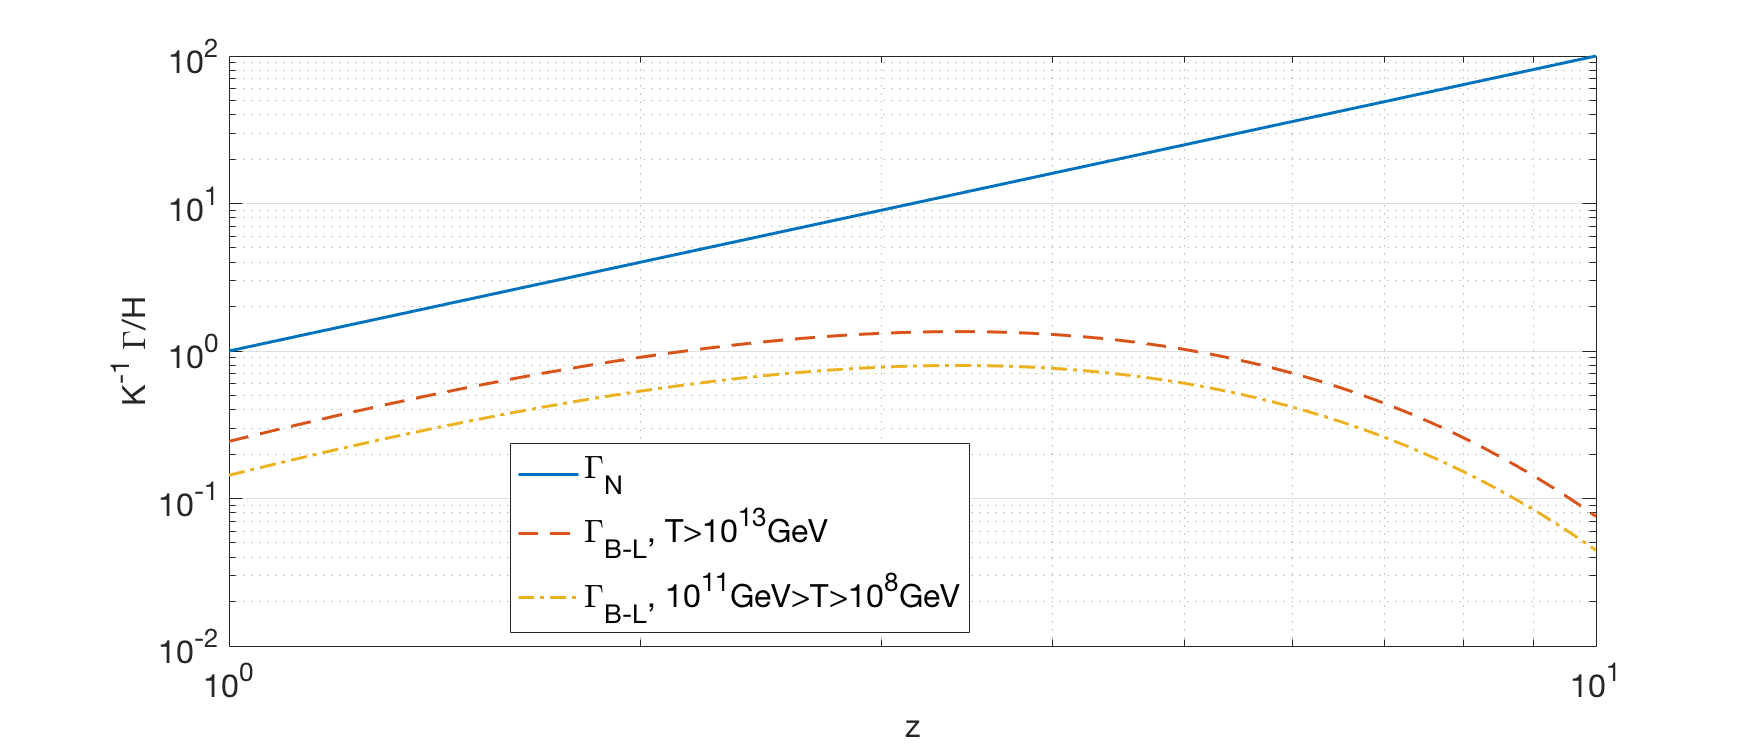
\includegraphics[width=0.7\linewidth]{Images/rates}
	\caption{}
	\label{fig:rates}
\end{figure}
